\documentclass[11pt]{article}

\usepackage[portuguese]{babel}
\usepackage[utf8]{inputenc}
\usepackage{amsmath}
\usepackage{graphicx}
\usepackage{float}
\usepackage{subfig}
\usepackage{fixltx2e}
\usepackage[bottom]{footmisc}
\usepackage{color}
\usepackage[usenames,dvipsnames]{xcolor}
\usepackage[colorinlistoftodos]{todonotes}
\usepackage[font=footnotesize]{caption}
\usepackage{relsize}

\numberwithin{equation}{section}

\linespread{1.3}
\usepackage{indentfirst}
\usepackage[top=2cm, bottom=2cm, right=2.25cm, left=2.25cm]{geometry}
\addto\captionsportuguese{\renewcommand{\contentsname}{Índice}}

\begin{document}

\begin{titlepage}
\begin{center}

\hfill \break
\hfill \break


\includegraphics[width=0.3\textwidth]{./logo}~\\[1cm]

\textsc{\LARGE Instituto Superior Técnico}\\[0.25cm]
\textsc{\Large Mestrado Integrado em Engenharia Electrotécnica e de Computadores}\\[1.8cm]
\textsc{\huge Sistemas Integrados Analógicos}\\[0.25cm]

{\huge \bfseries \textit{Design} de um Amplificador \\[1cm]}

\begin{tabular}{ l l }
João Bernardo Sequeira de Sá & \hspace{2mm} n.º 68254 \\
Maria Margarida Dias dos Reis & \hspace{2mm} n.º 73099 \\
Nuno Miguel Rodrigues Machado & \hspace{2mm} n.º 74236
\end{tabular}

\vfill

{\large Lisboa, 1 de Maio de 2015} 

\end{center}
\end{titlepage}

\pagenumbering{gobble}
\clearpage

\tableofcontents
\pagebreak

\clearpage
\pagenumbering{arabic}

\section{Introdução}

Pretende-se projectar um amplificador \textit{folded cascode} CMOS OTA de dois andares de acordo com as especificações da seguinte tabela.

\begin{table}[H]
	\centering
	\caption{Características do amplificador a projectar.}
	\vspace{-1.5mm}
	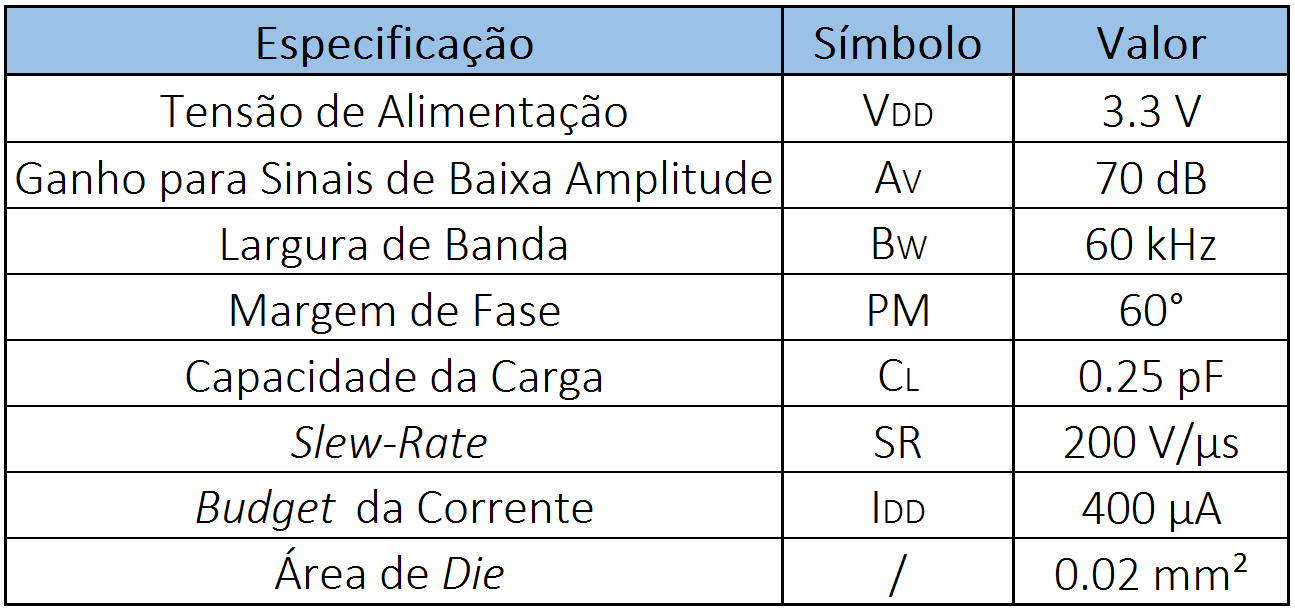
\includegraphics[keepaspectratio=true, scale=0.45]{teoricas/tabela1}
\end{table}

O circuito de ponto de partida para a realização do projecto é apresentado de seguida.

\begin{figure}[H]
	\centering
	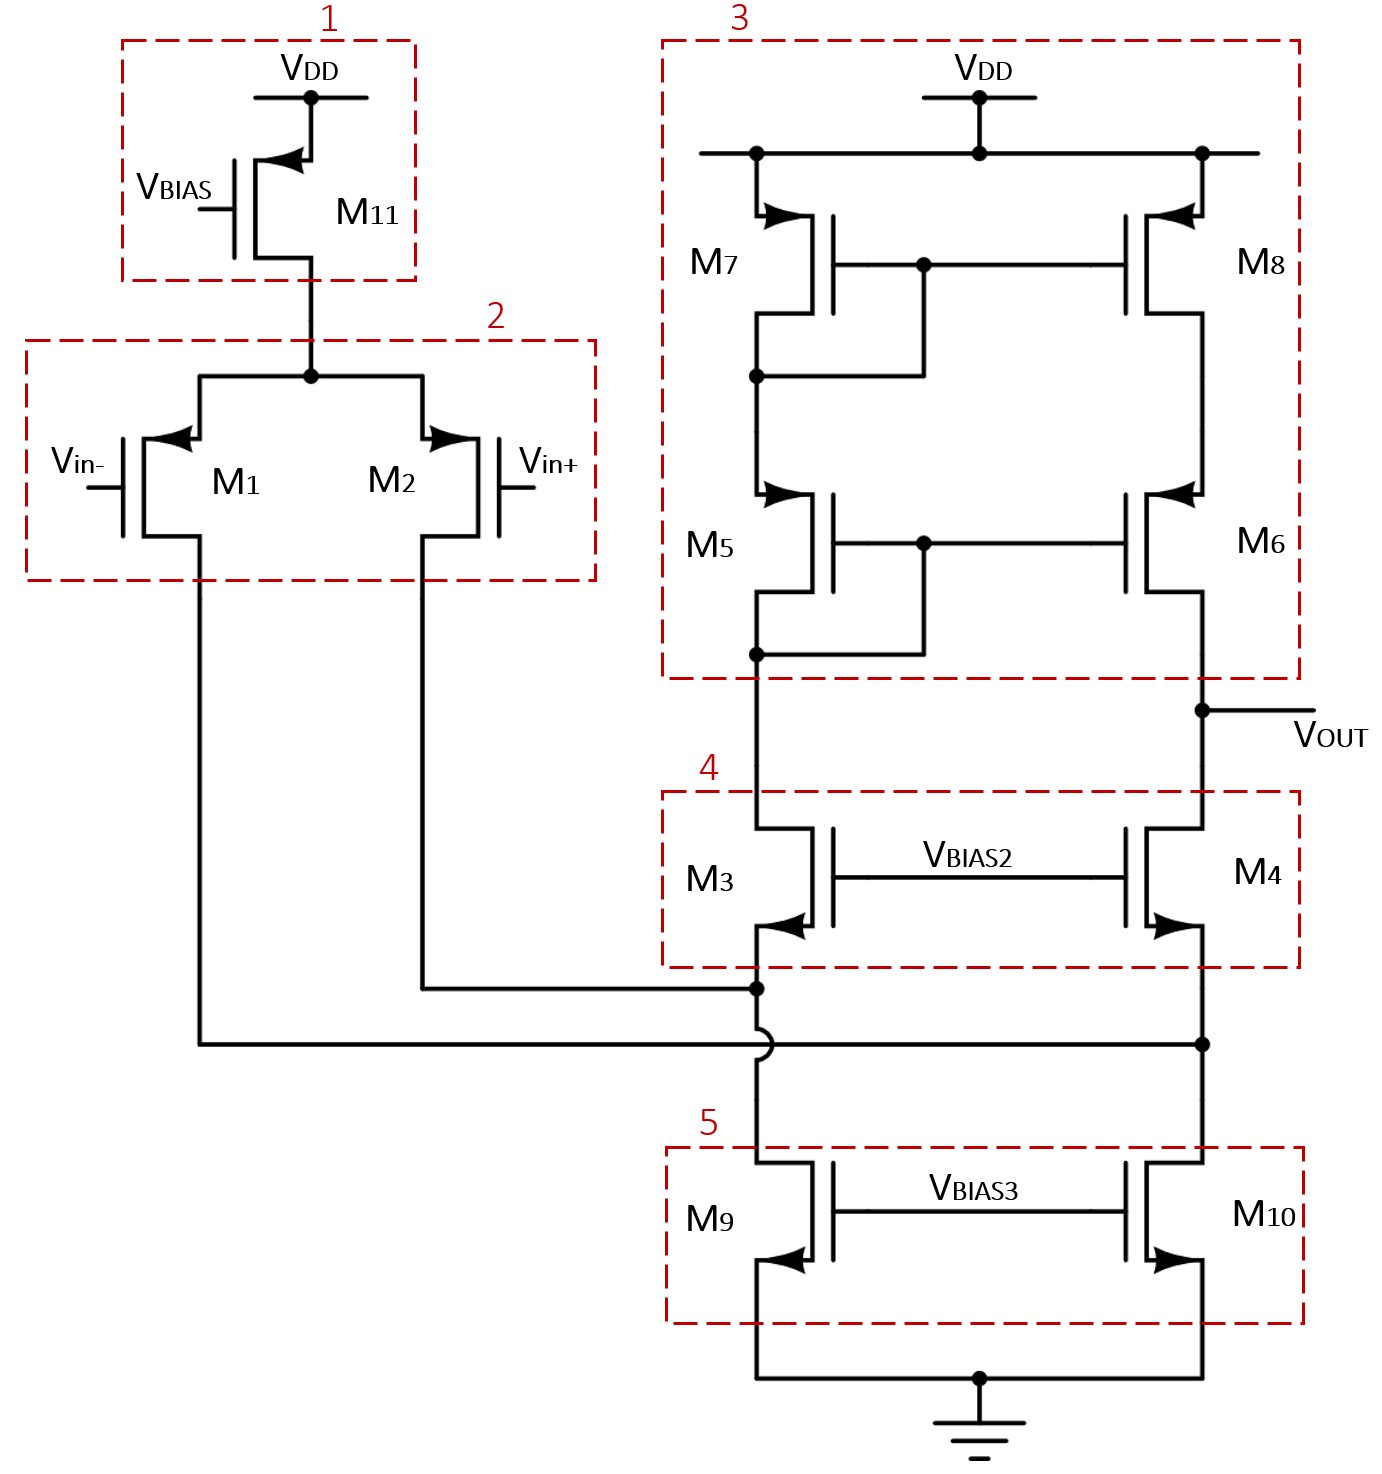
\includegraphics[keepaspectratio=true, scale=0.50]{teoricas/circuito1}
	\vspace{-0.5em}
	\caption{Circuito do amplificador a projectar.}
	\vspace{-0.8em}
\end{figure} 

\pagebreak

\section{Funcionamento Teórico do Circuito}

\todo{introducao teorica do OTA}

Analisando o circuito da Figura 1 em pormenor identificam-se 5 blocos, sendo importante analisar a função de cada um, para que melhor se possa compreender o funcionamento e comportamento do circuito na sua totalidade. 

O Bloco 1 representa o transístor responsável pela polarização do circuito. O Bloco 2 representa um par diferencial PMOS. O Bloco 3 corresponde a um espelho de corrente \textit{cascode} básico do tipo PMOS. O Bloco 4 actua como isolamento. O Bloco 5 funciona como fonte de corrente que ``puxa'' sempre $I$ (corrente de M\textsubscript{11}) para o \textit{ground}.

Relativamente ao par diferencial, o circuito pode funcionar de acordo com três situações:

\begin{itemize}
	\vspace{-3mm}
	\item $v_{in-} = v_{in+} \rightarrow$ situação 1
	\vspace{-1.5mm}
	\item $v_{in-} > v_{in+} \rightarrow$ situação 2
	\vspace{-1.5mm}
	\item $v_{in-} < v_{in+} \rightarrow$ situação 3
\end{itemize}

Na situação 1, cada transístor do par diferencial, M\textsubscript{1} e M\textsubscript{2}, tem metade da corrente que passa em M\textsubscript{11} e o circuito apresenta o seguinte comportamento.

\begin{figure}[H]
	\centering
	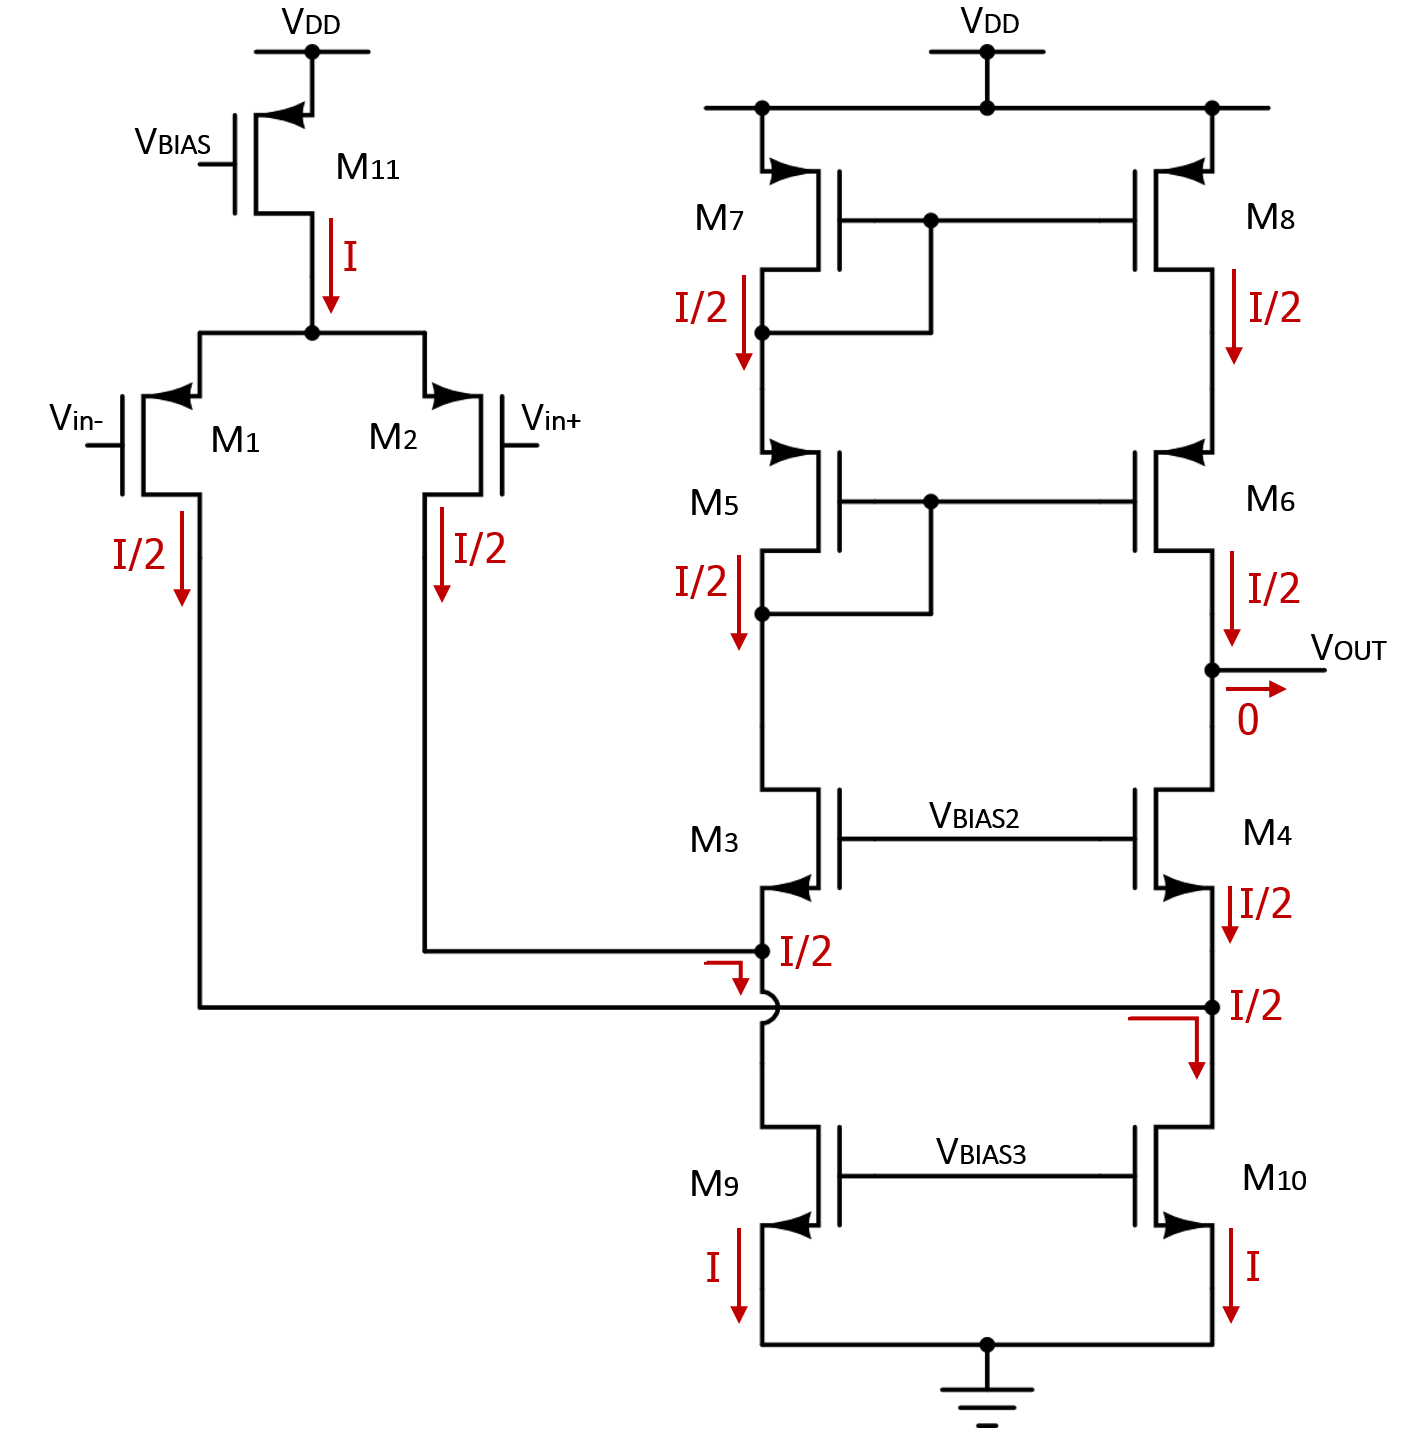
\includegraphics[keepaspectratio=true, scale=0.50]{teoricas/situacao1}
	\vspace{-0.5em}
	\caption{Funcionamento do circuito na situação 1.}
	\vspace{-0.8em}
\end{figure} 

Considerando agora o extremo da situação 2, a tensão na \textit{gate} de M\textsubscript{1} toma o valor máximo da fonte de tensão que polariza esse transístor e a tensão na \textit{gate} de M\textsubscript{2} é nula. Assim, o circuito apresenta o seguinte comportamento.

\begin{figure}[H]
	\centering
	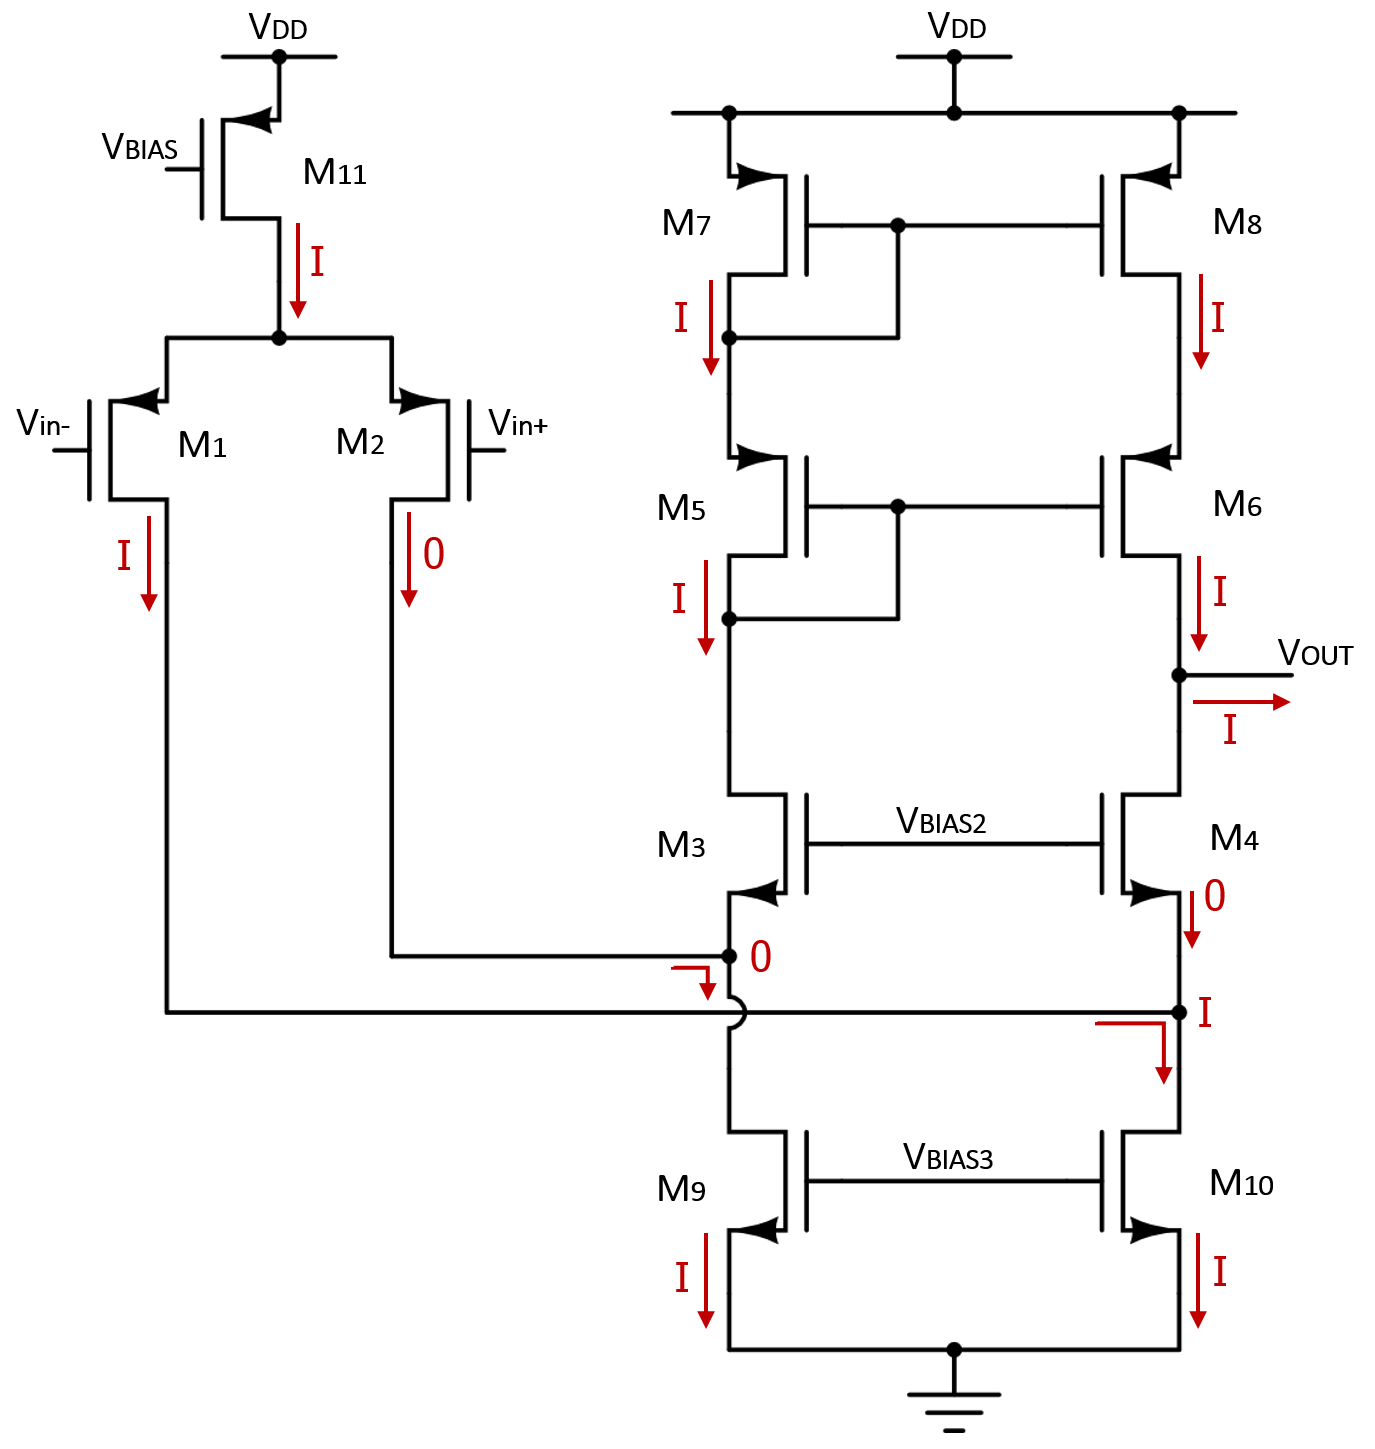
\includegraphics[keepaspectratio=true, scale=0.50]{teoricas/situacao2}
	\vspace{-0.5em}
	\caption{Funcionamento do circuito no extremo da situação 2.}
	\vspace{-0.8em}
\end{figure} 

Considerando agora o extremo da situação 3, a tensão na \textit{gate} de M\textsubscript{2} toma o valor máximo da fonte de tensão que polariza esse transístor e a tensão na \textit{gate} de M\textsubscript{1} é nula. Assim, o circuito apresenta o seguinte comportamento.

\begin{figure}[H]
	\centering
	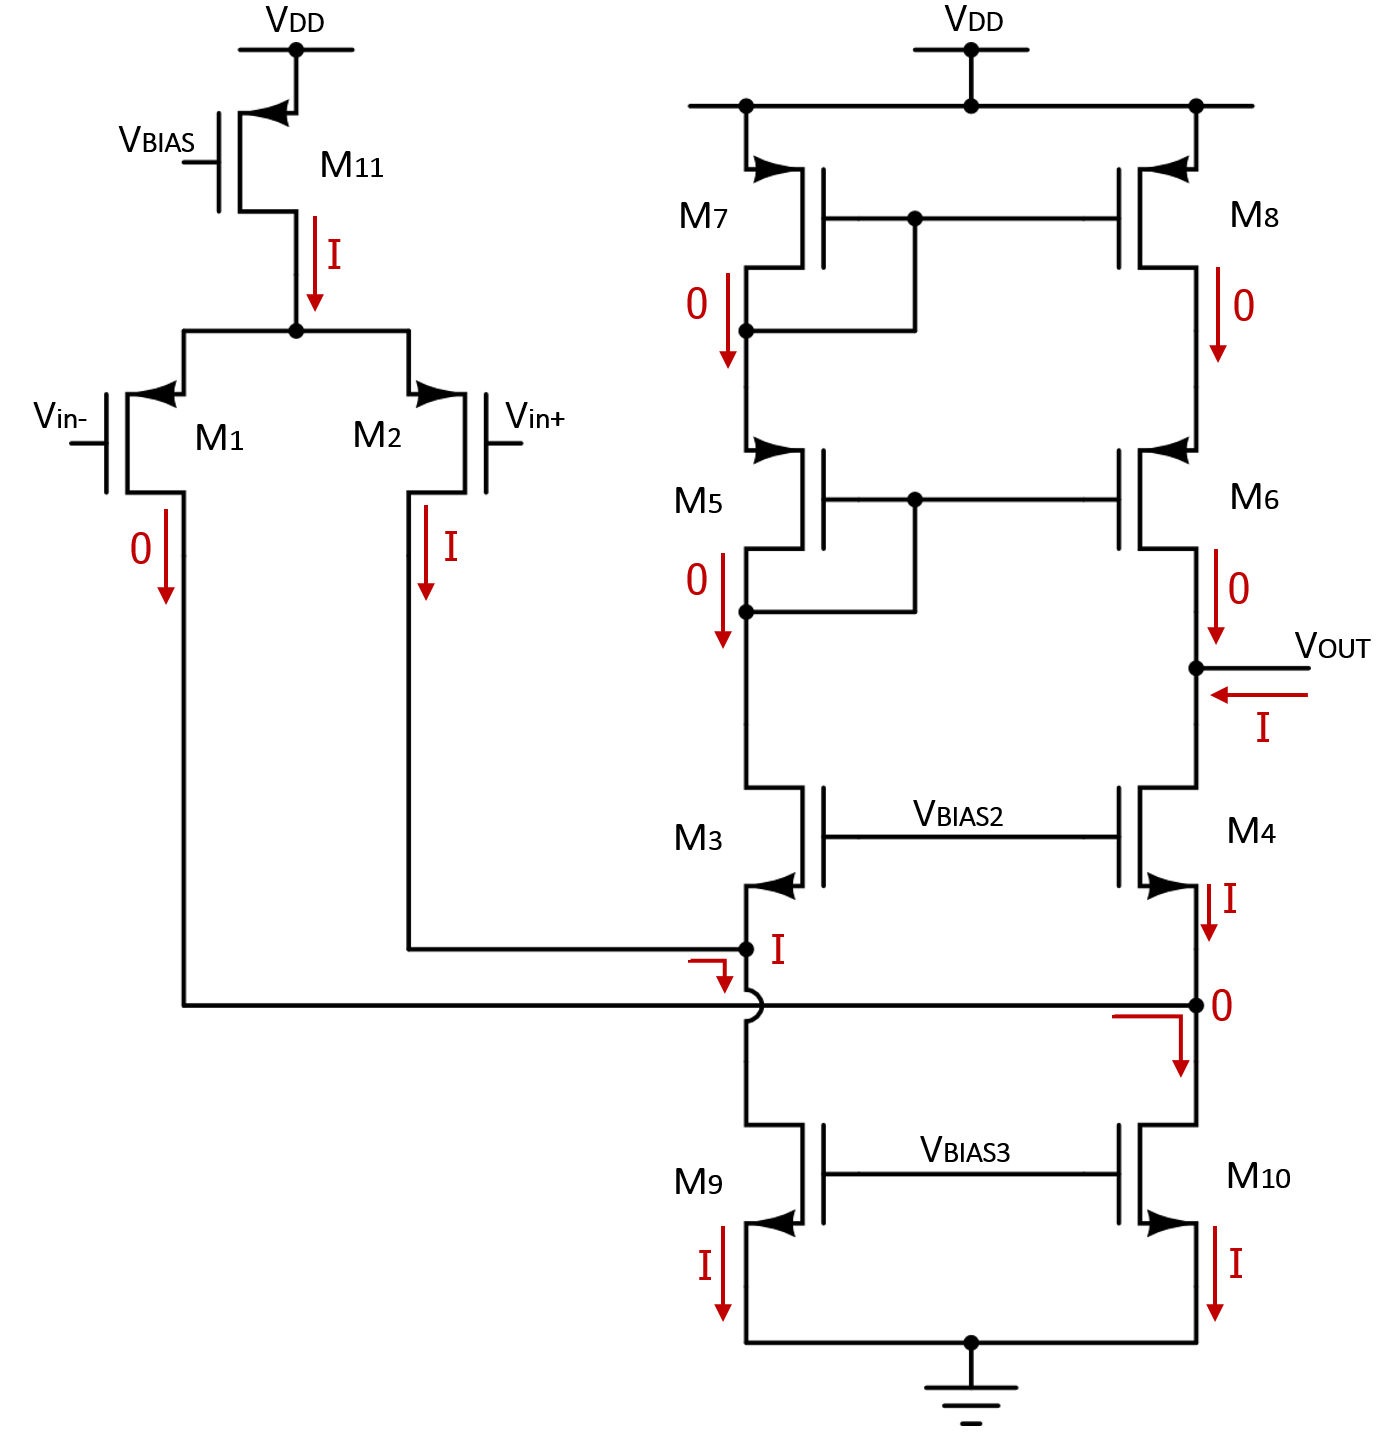
\includegraphics[keepaspectratio=true, scale=0.50]{teoricas/situacao3}
	\vspace{-0.5em}
	\caption{Funcionamento do circuito no extremo da situação 3.}
	\vspace{-0.8em}
\end{figure} 

\section{Dimensionamento dos Transístores}

A primeira fase no projecto do amplificador passou por decidir as dimensões dos vários transístores. Sabe-se que a dimensão de um transístor é dada pelos parâmetros $W$ (\textit{width} - largura) e $L$ (\textit{lenght} - comprimento). 

\subsection{\textit{Slew-Rate}}

Para efectuar o primeiro dimensionamento dos transístores teve-se em consideração o critério da \textit{slew-rate}, onde se pretende atingir um valor de 200 V/$\mu$s.

O valor de $L$ ficou decidido à partida como sendo 1 $\mu$m para todos os transístores do circuito, isto porque se tem como \textit{rule of thumb} que, para se evitar o efeito de modulação do comprimento do canal, o valor de $L$ deve ser maior ou igual a 1 $\mu$m. O valor de $W$ pode ser calculado recorrendo à equação que determina a corrente num transístor. Para um transístor do tipo P a corrente é dada por

\vspace{-3mm}
\begin{equation}
I_{D} = \frac{1}{2}\mu_{n}C_{ox}\times \left(\frac{W}{L}\right) \times \left(V_{GS}-V_{TH}^2\right) = k_P \times \left(\frac{W}{L}\right) \times V_{OD}^2,
\label{eq:corrente}
\end{equation}

\vspace{1mm}
sendo que para um transístor do tipo N troca o valor do factor de ganho, em vez de $k_P$ tem-se $k_N$.

Da equação anterior pretende-se determinar o valor de $W$ dos vários transístores, sendo então necessário saber o valor de $L$ (já determinado anteriormente), o valor da corrente que passa nos transístores, $I_{D}$, o valor de $k$ e o valor da tensão de \textit{overdrive}, $V_{OD}$.

O valor da tensão de \textit{overdrive} definiu-se como sendo de 0.2 V para todos os transístores. Este valor deriva de outra \textit{rule of thumb} que indica que se deve escolher para $V_{OD}$ um valor de 0.2V - menos do que isso e fica-se demasiado sensível a $V_{TH}$ e mais do que isso e fica-se com pouca margem de saturação, que é uma medida do quão dentro da saturação se está, sendo calculada por $V_{DS} - V_{OD}$.

O valor de $k$ pode ser obtido com recurso aos \textit{process parameters}, sendo de referir que o valores que se retiram das \textit{datasheets} representam apenas $\mu_{n}C_{ox}$, pelo que têm de ser multiplicados por $1/2$ para que se obtenha o factor de ganho final, como se pode ver na próxima equação, para o caso de um transístor do tipo P:

\vspace{-3mm}
\begin{equation}
k_P = \frac{1}{2}\mu_{n}C_{ox} = \frac{1}{2} \times KP_P.
\end{equation}

\vspace{1mm}
Os valores já conhecidos que ajudam a obter o valor de $W$ através da equação (2.1) encontram-se esquematizados na seguinte tabela.

\begin{table}[H]
	\centering
	\caption{Valores especificados para algumas das características que definem os transístores.}
	\vspace{-1.5mm}
	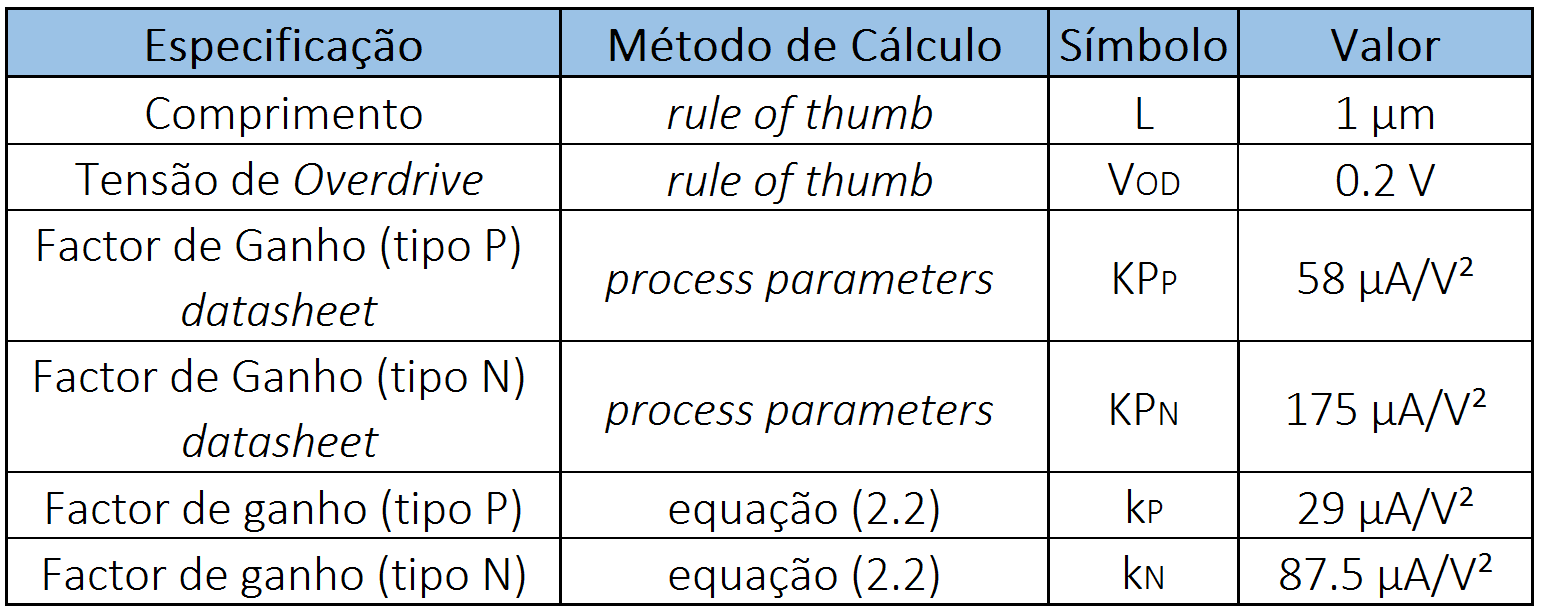
\includegraphics[keepaspectratio=true, scale=0.45]{teoricas/tabela2}
\end{table}

Para determinar os valores das correntes que passam nos vários transístores começou-se por determinar a corrente máxima à saída do circuito. Existe uma relação entre a \textit{slew-rate}, SR, e a corrente de saída máxima, $I_{out_{max}}$ expressa por

\vspace{-3mm}
\begin{equation}
\text{SR} = \frac{I_{out_{max}}}{C_L},
\end{equation}

\vspace{1mm}
que nos permite concluir que quanto maior for a corrente de saída, mais depressa é carregado o condensador que constitui a carga.

Com os valores da Tabela 1 obtém-se:

\vspace{-3mm}
\begin{equation}
\text{SR} = \frac{I_{out_{max}}}{C_L} \leftrightarrow I_{out_{max}} = 200 \times 0.25 \times 10^{-6}~\text{A} = 50~\mu \text{A}.
\end{equation}

\vspace{1mm}
Analisando as Figuras 3 a 4 percebe-se que a corrente $I_{out_{max}}$ corresponde a $I/2$, pelo que o valor máximo de $I$ corresponde a 100 $\mu$A. O dimensionamento dos transístores foi feito tendo em conta o ponto de funcionamento em repouso (PFR), situação 1, de acordo com

\vspace{-3mm}
\begin{equation}
W_P  = \frac{I_{D} \times L}{k_P \times V_{OD}^2} \rightarrow \text{transístor tipo PMOS};
\end{equation}
\vspace{1mm}
\begin{equation}
W_N  = \frac{I_{D} \times L}{k_N \times V_{OD}^2} \rightarrow \text{transístor tipo NMOS}.
\end{equation}

\vspace{1mm}
Os valores obtidos para a \textit{width} dos vários transístores apresenta-se na tabela seguinte. De notar que os valores foram arredondados ao inteiro mais próximo.

\begin{table}[H]
	\centering
	\caption{Valores de $W$ dos transístores que constituem o circuito, calculados em função do PFR.}
	\vspace{-1.5mm}
	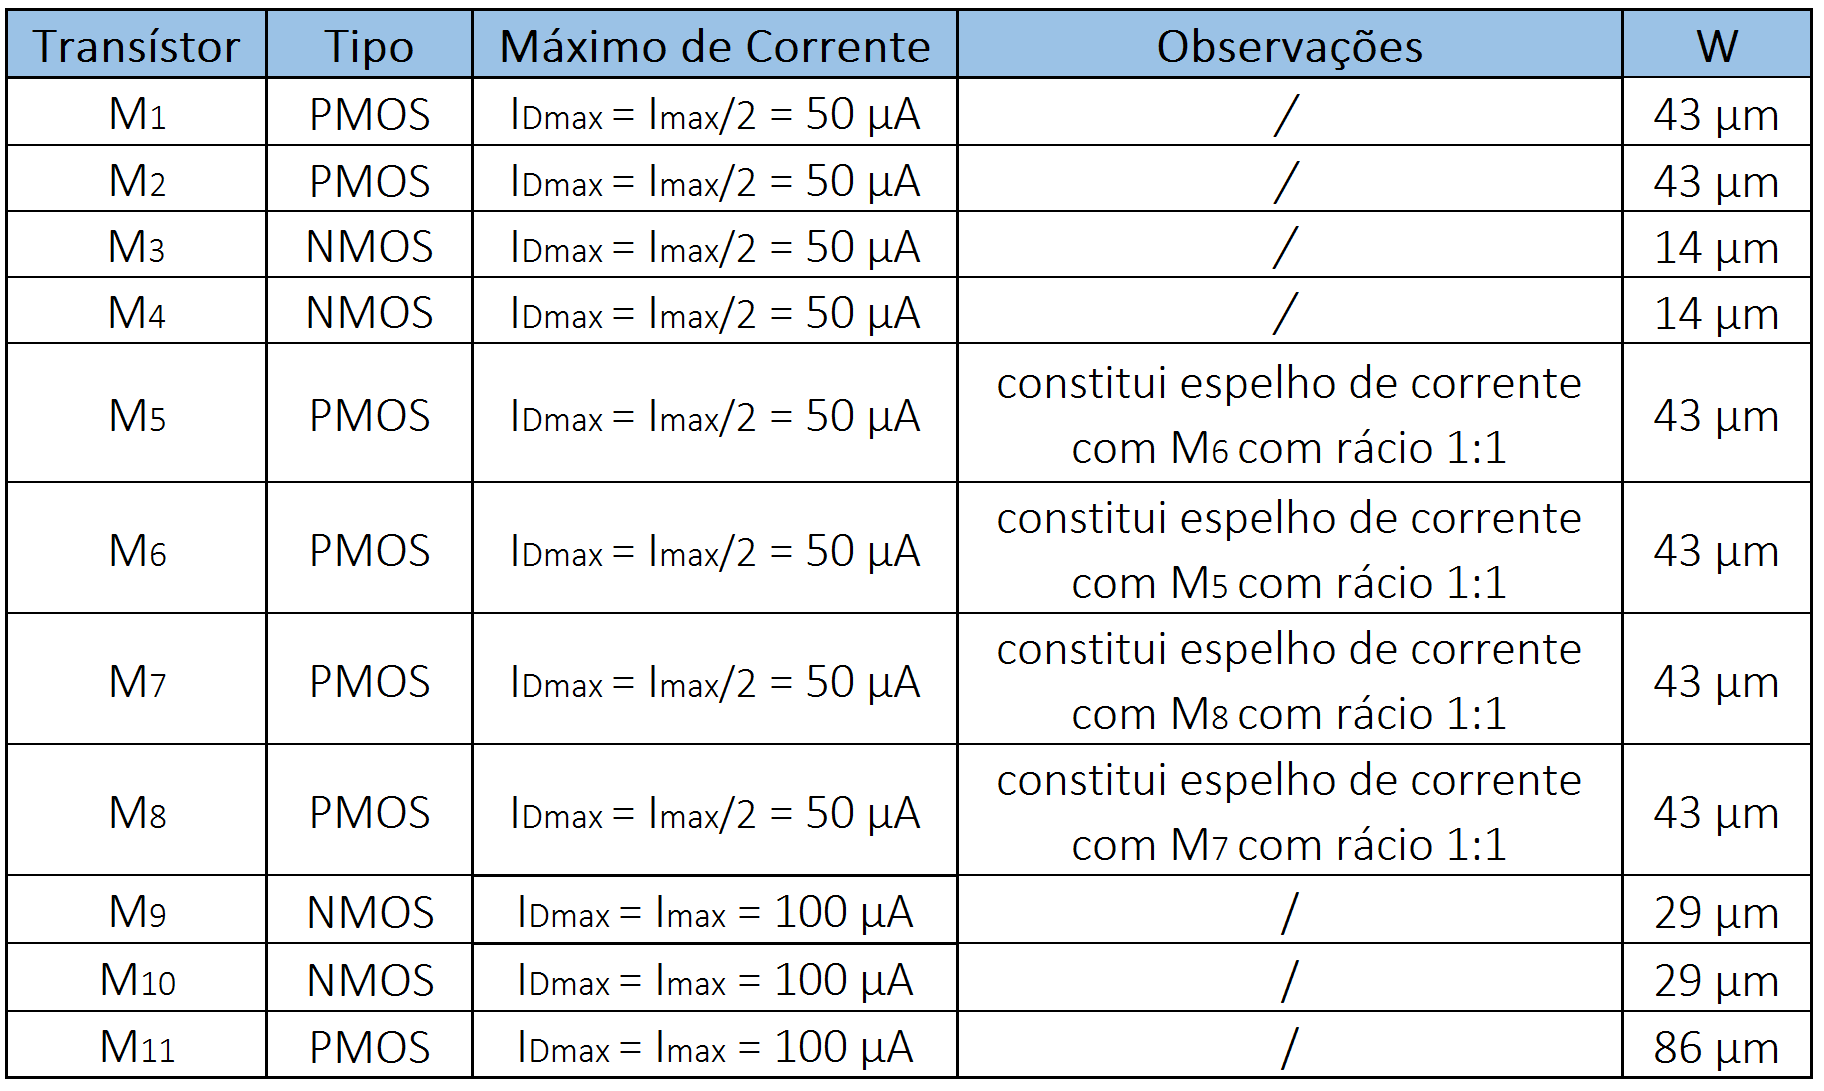
\includegraphics[keepaspectratio=true, scale=0.45]{teoricas/valoresW2}
\end{table}

De referir que os transístores M\textsubscript{5} e M\textsubscript{6} têm as mesmas dimensões, tal como pretendido, pois formam um espelho de corrente que tem como rácio 1:1. O mesmo se aplica aos transístores M\textsubscript{7} e M\textsubscript{8}.

Com o dimensionamento dos transístores feito procede-se a uma primeira simulação do circuito, com o intuito de verificar o seu funcionamento. Porém, antes de simular o circuito alterou-se a sua polarização, para que em vez de ser feita em tensão seja feita em corrente. Isto é feito porque uma polarização em corrente permite ter mais controlo, sendo que quando é feita em tensão não se tem garantias dos valores pretendidos.  

Assim, o circuito da Figura 1 foi alterado para o apresentado de seguida.

\begin{figure}[H]
	\centering
	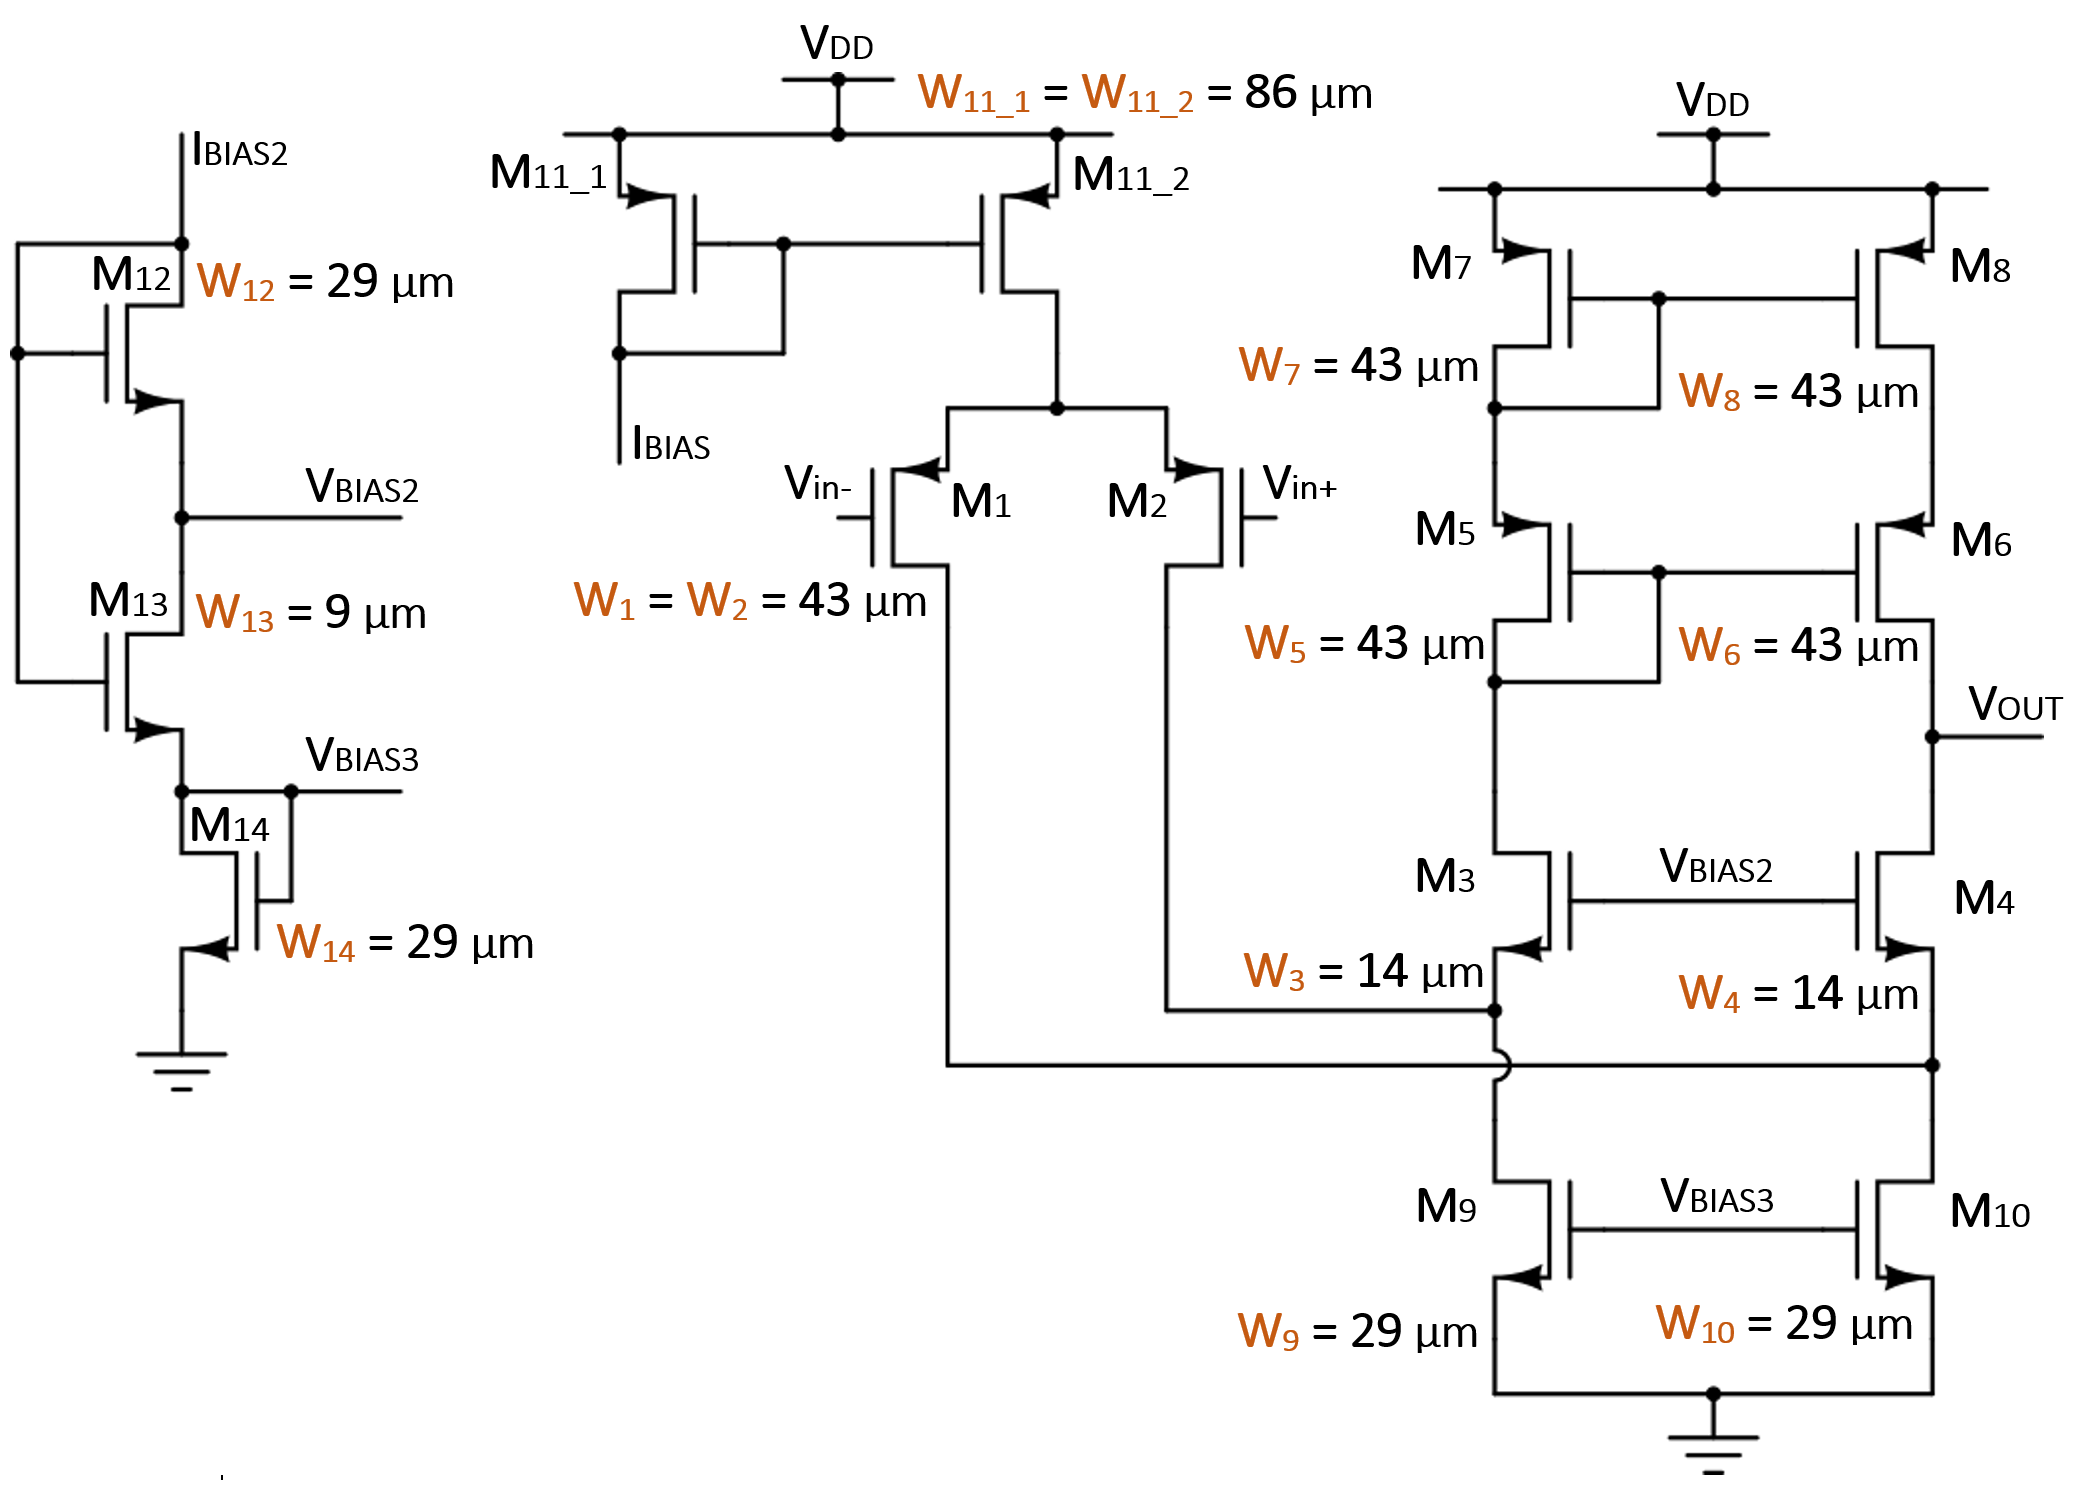
\includegraphics[keepaspectratio=true, scale=0.55]{teoricas/primeirasimul}
	\vspace{-0.5em}
	\caption{Primeiro circuito de simulação do amplificador.}
	\vspace{-0.8em}
\end{figure} 

Na figura anterior pode-se ver o valor de $W$ utilizado nos vários transístores, sendo que para todos o valor de $L$ é de 1 $\mu$m.

Como se pode ver, o transístor M\textsubscript{11} que é originalmente polarizado em tensão com $V_{BIAS}$, Bloco 1, foi substituído por um espelho de corrente básico que é polarizado em corrente com $I_{BIAS}$. A polarização feita com recurso a $V_{BIAS_{2}}$ e $V_{BIAS_{3}}$ foi tanbém alterada para passar a ser feita em corrente com $I_{BIAS_{2}}$, através de um espelho de corrente \textit{cascode} \textit{low-voltage}. O valor de $I_{BIAS}$ e de $I_{BIAS_{2}}$ é de 100 $\mu$A.

De notar que os transístores M\textsubscript{11\textsubscript{1}} e M\textsubscript{11\textsubscript{2}} têm a mesma dimensão que aquela que foi determinada para M\textsubscript{11}, uma vez que a corrente que os atravessa é também 100 $\mu$A e são do tipo PMOS. Já os transístores M\textsubscript{12} e M\textsubscript{14} têm a mesma dimensão que M\textsubscript{9} e M\textsubscript{10}, uma vez que a corrente que os atravessa é também 100 $\mu$A e são do tipo NMOS. O transístor M\textsubscript{13}, de acordo com o funcionamento teórico de um espelho de corrente \textit{cascode} \textit{low-voltage}, deve ter um $W$ 3 vezes inferior ao de M\textsubscript{12}, assim como deve funcionar sempre no tríodo, o que implica uma \textit{width} de 9 $\mu$m.

Na Figura 6 encontra-se o \textit{schematic} criado no Cadence correspondente ao da Figura 5.

\begin{figure}[H]
	\centering
	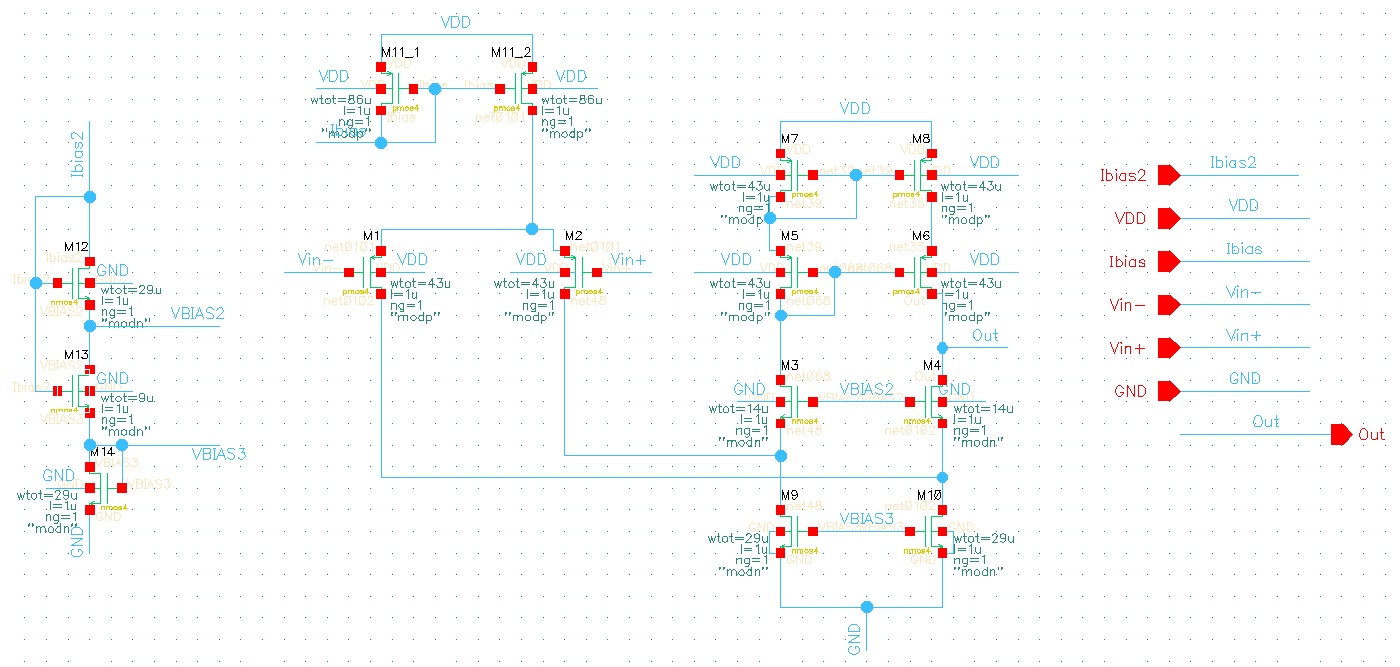
\includegraphics[keepaspectratio=true, scale=0.70]{exps/Woriginais}
	\vspace{-0.5em}
	\caption{\textit{Schematic} do circuito criado para a primeira simulação.}
	\vspace{-0.8em}
\end{figure} 

Com o \textit{schematic} anterior projectou-se um símbolo e criou-se um novo \textit{schematic} de \textit{testbench}, como se pode ver na Figura 7.

\begin{figure}[H]
	\centering
	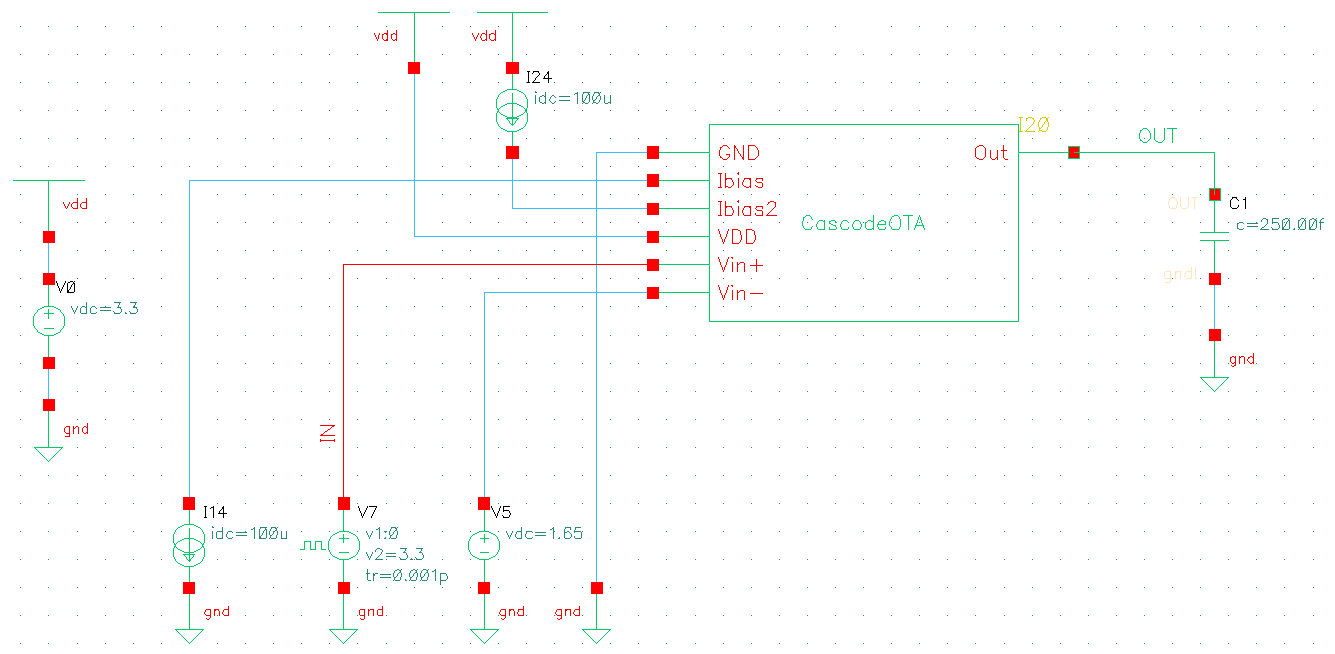
\includegraphics[keepaspectratio=true, scale=0.47]{exps/testbench}
	\vspace{-0.5em}
	\caption{\textit{Schematic} do \textit{testbench} que permite simular o circuito.}
	\vspace{-0.8em}
\end{figure} 

Recorrendo ao circuito da figura anterior efectuou-se uma análise \textit{transient} durante 2 ms. Para verificar se o circuito funciona como pretendido otpou-se por verificar se todos os transístores do amplificador tem a corrente $I_D$ pretendida, ou seja, de acordo com a Figura 1, e se estão na região de saturação.

\begin{figure}[H]
	\centering
	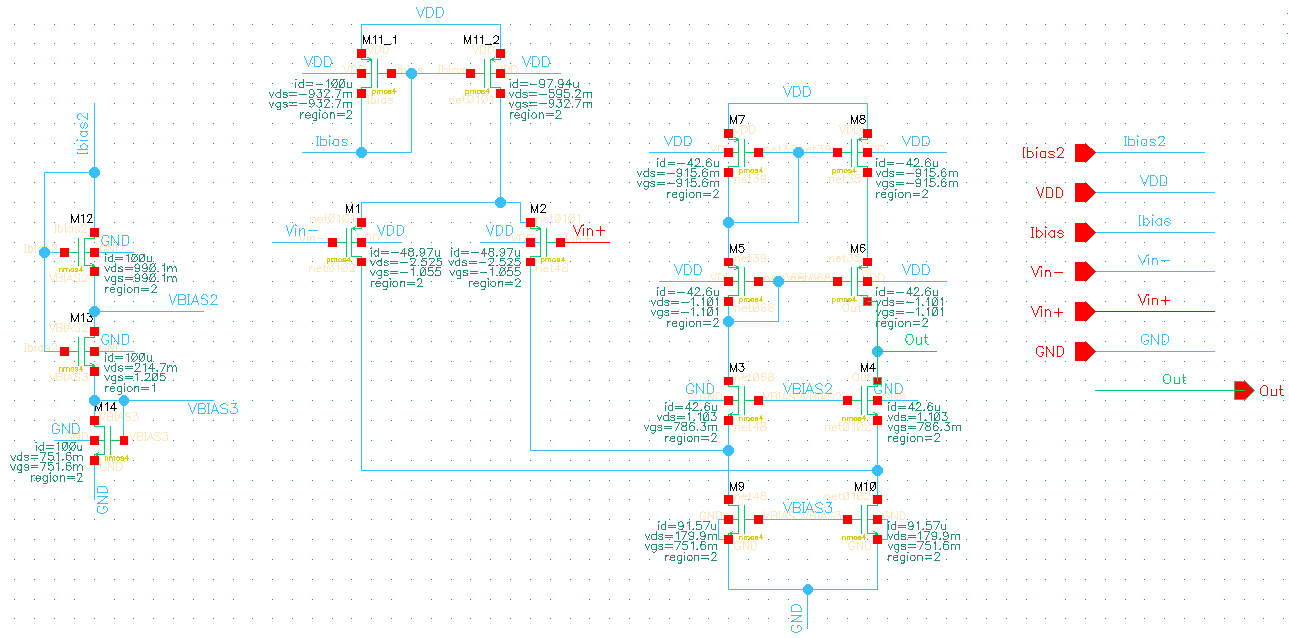
\includegraphics[keepaspectratio=true, scale=0.85]{exps/PFRoriginais}
	\vspace{-0.5em}
	\caption{Valores do PFR do \textit{schematic} da Figura 6.}
	\vspace{-0.8em}
\end{figure} 

A região de funcionamento dos transístores pode ser vista na secção \textit{region}: 0 implica que o transístor está ao corte, 1 que está no tríodo, 2 que está na zona de saturação e 3 na região de \textit{subthreshold}.

Como se pode ver, todos os transístores do amplificador estão na região 2, tal como pretendido, assim como os que polarizam através de $I_{BIAS}$. Os transístores M\textsubscript{12} e M\textsubscript{14} do espelho de corrente \textit{cascode} \textit{low-voltage} estão também saturados e o transístor M\textsubscript{13} está no tríodo, tal como se queria.

Porém, apesar de os transístores estarem a funcionar na zona correcta, o valor das suas correntes está ligeiramente afastado do pretendio. Os transístores M\textsubscript{3}, M\textsubscript{4}, M\textsubscript{5}, M\textsubscript{6}, M\textsubscript{7} e M\textsubscript{8} deveriam ter um valor de $I_D$ de 50 $\mu$A, sendo, no entanto, o valor registado pela simulação de 42.6 $\mu$A. Para os transístores M\textsubscript{9} e M\textsubscript{10} esperava-se um valor de $I_D$ de 100 $\mu$A, sendo, no entanto, o valor registado pela simulação de 91.57 $\mu$A. As correntes do espelho de corrente básico estão de acordo com o esperado, sendo que os transístores M\textsubscript{1} e M\textsubscript{2} têm um valor de corrente de 48.97 $\mu$A, um valor próximo do esperado de 50 $\mu$A.

Até agora, para efectuar o dimensionamento dos transístores o critério que se teve em consideração foi a \textit{slew-rate}. Assim, com recurso à calculadora do Cadence calculou-se o seu valor, sendo este de $170.7\times10^6$ V/segundo $\leftrightarrow 170.7$ V/$\mu$s. O valor pretendido é de 200 V/$\mu$s, verificando-se então alguma diferença entre os dois valores.

Relativamente aos valores de $V_{GS}$ para os vários transístores, os valores teóricos esperados foram calculados com base nos \textit{process parameters} da seguinte forma:

\vspace{-3mm}
\begin{equation}
V_{TH_{P}} \approx 0.6 V \rightarrow V_{GS} = V_{OD} + V_{TH_{N}} = 0.2 + 0.6 = 0.8 V \rightarrow \text{transístor tipo PMOS};
\end{equation}
\begin{equation}
V_{TH_{N}} \approx 0.5 V \rightarrow V_{GS} = V_{OD} + V_{TH_{N}} = 0.2 + 0.5 = 0.7 V \rightarrow \text{transístor tipo NMOS}.
\end{equation}

\vspace{1mm}
Na Figura 6 pode-se verificar \todo{comentarios sobre os valores de vgs}

Face à ligeira discrepância nos valores obtidos para a corrente nos vários transístores e para a \textit{slew-rate}, decidiu-se proceder a um ajuste nas dimensões dos transístores para se obter valores mais próximos dos esperados. Este ajuste foi feito ao nível dos transístores M\textsubscript{3} e M\textsubscript{4} pois, ao aumentar as suas dimensões faz-se variar as suas tensões $V_{GS}$, e como tal $V_{BIAS_{2}}$, o que resulta num aumento da tensão $V_{DS}$ de M\textsubscript{9}, que por sua vez faz aumentar a corrente daquele ramo.

O ajuste feito nesses dois transístores passou por aumentar o seu rácio $W/L$ para o dobro, ou seja, o valor de $W$ passou de 14$\mu$m para 28$\mu$m. À primeira vista não parecer ser um ajuste fino, no entanto, está associado à existência de um efeito de segunda-ordem.

De facto, quando se é mais criterioso, a corrente de um transístor não é calculada de acordo com a equação (2.1), mas sim de acordo com

\vspace{-3mm}
\begin{equation}
I_{D} = \frac{1}{2}\mu_{n}C_{ox}\times \left(\frac{W}{L}\right) \times \left(V_{GS}-V_{TH}^2\right) \times \left(1+\lambda V_{DS}\right) = k_P \times \left(\frac{W}{L}\right) \times V_{OD}^2 \times \left(1+\lambda V_{DS}\right).
\end{equation}

\vspace{1mm}
Como se pode ver, sobre o valor da corrente existe um efeito de segunda-ordem com a introdução da parcela $\left(1+\lambda V_{DS}\right)$. Assim se explica que, quando o valor de $W$ de M\textsubscript{3} e M\textsubscript{4} passa para o dobro, a corrente nos transístores aumenta em aproximadamente 7$\mu$A, conseguindo-se obter o valor desejado de 50$\mu$A.

Os transístores M\textsubscript{9} e M\textsubscript{10} também viram as suas dimensões alteradas e, após um ajuste fino, o seu valor de $W$ passou de 29$\mu$m para 30$\mu$m. Fizeram-se mais ajustes finos, sendo que o transístor M\textsubscript{12} passou para um $W$ de 28$\mu$m e o transístor M\textsubscript{13} para um $W$ de 7$\mu$m.

Na Figura 9 apresenta o circuito com o ajuste nas dimensões dos transístores.

\begin{figure}[H]
	\centering
	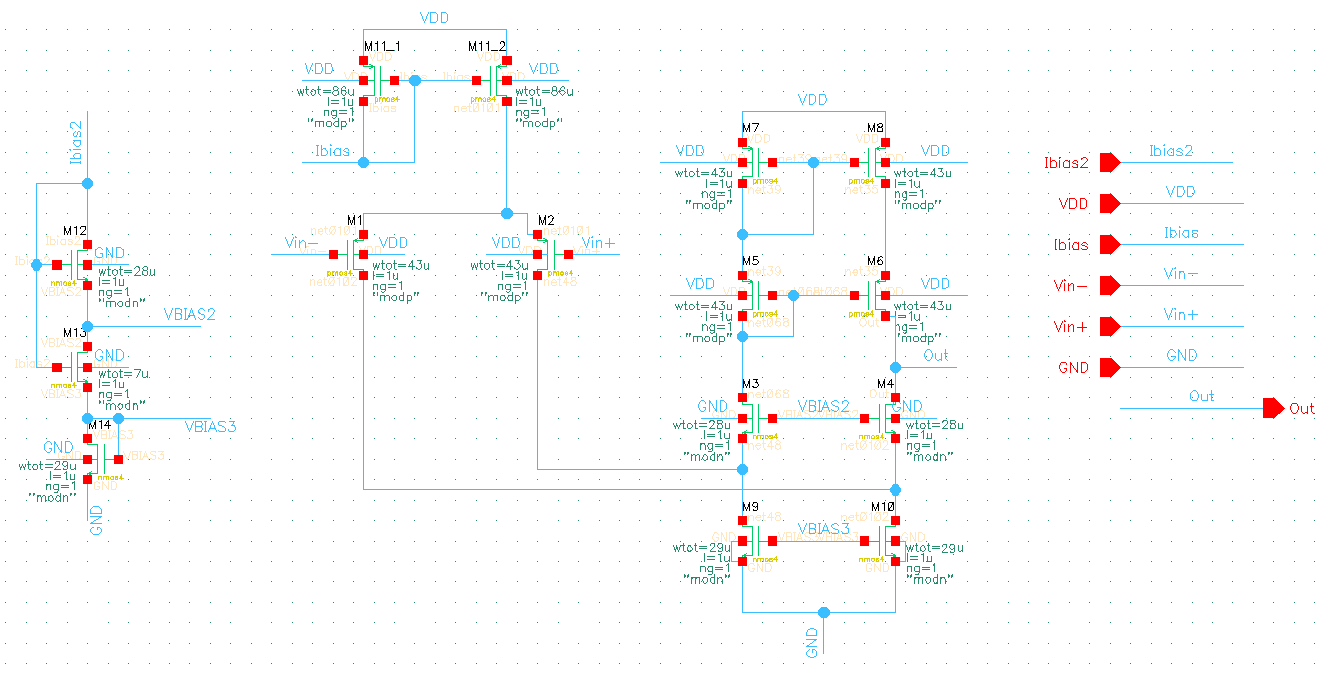
\includegraphics[keepaspectratio=true, scale=0.70]{exps/Wajustados}
	\vspace{-0.5em}
	\caption{\textit{Schematic} do circuito com os valores de $W$ ajustados.}
	\vspace{-0.8em}
\end{figure}

\begin{figure}[H]
	\centering
	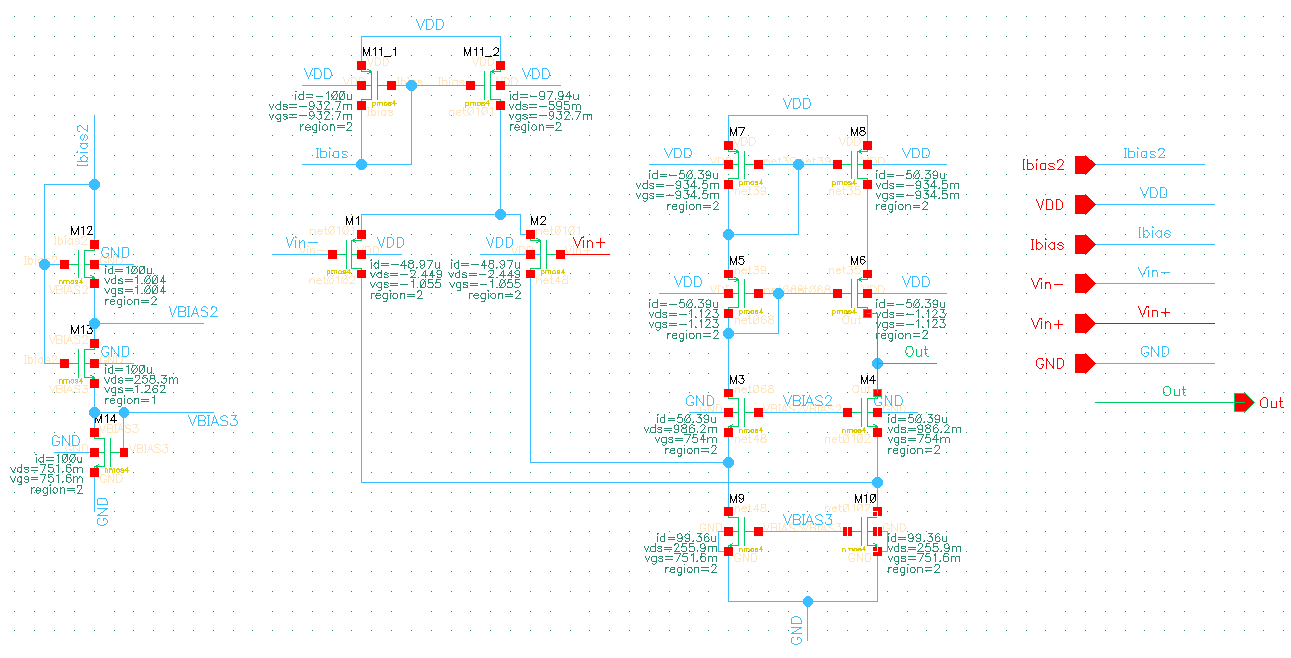
\includegraphics[keepaspectratio=true, scale=0.85]{exps/PFRajustados}
	\vspace{-0.5em}
	\caption{Valores do PFR do \textit{schematic} da Figura 9.}
	\vspace{-0.8em}
\end{figure}

Como se pode ver na figura anterior, o valor da corrente nos transístores M\textsubscript{3} a M\textsubscript{8} passou para 50.39$\mu$A, um valor muito próximo do pretendido de 50$\mu$A. Relativamente aos transístores M\textsubscript{9} e M\textsubscript{10}, passaram a ter uma corrente de 99.36$\mu$A, um valor também bastante próximo do pretendido de 100$\mu$A.

Face a estes ajustes mediu-se novamente o valor da \textit{slew-rate} para verificar se o critério já é cumprido. O valor medido foi de $199.9\times10^6$ V/segundo $\leftrightarrow 199.9$ V/$\mu$s, um valor que se considera óptimo.

Assim, o estado actual do circuito é apresentado de seguida. Na tabela da direita pode-se ver as especificações pretendidas e as que se verificam até ao momento, sendo que a verde se assinalam aquelas que se considera cumpridas e a vermelho aquelas que se pretende melhorar.

\begin{figure}[h]
	\centering
	\begin{minipage}[c]{0.58\textwidth}
		\begin{figure}[H]
			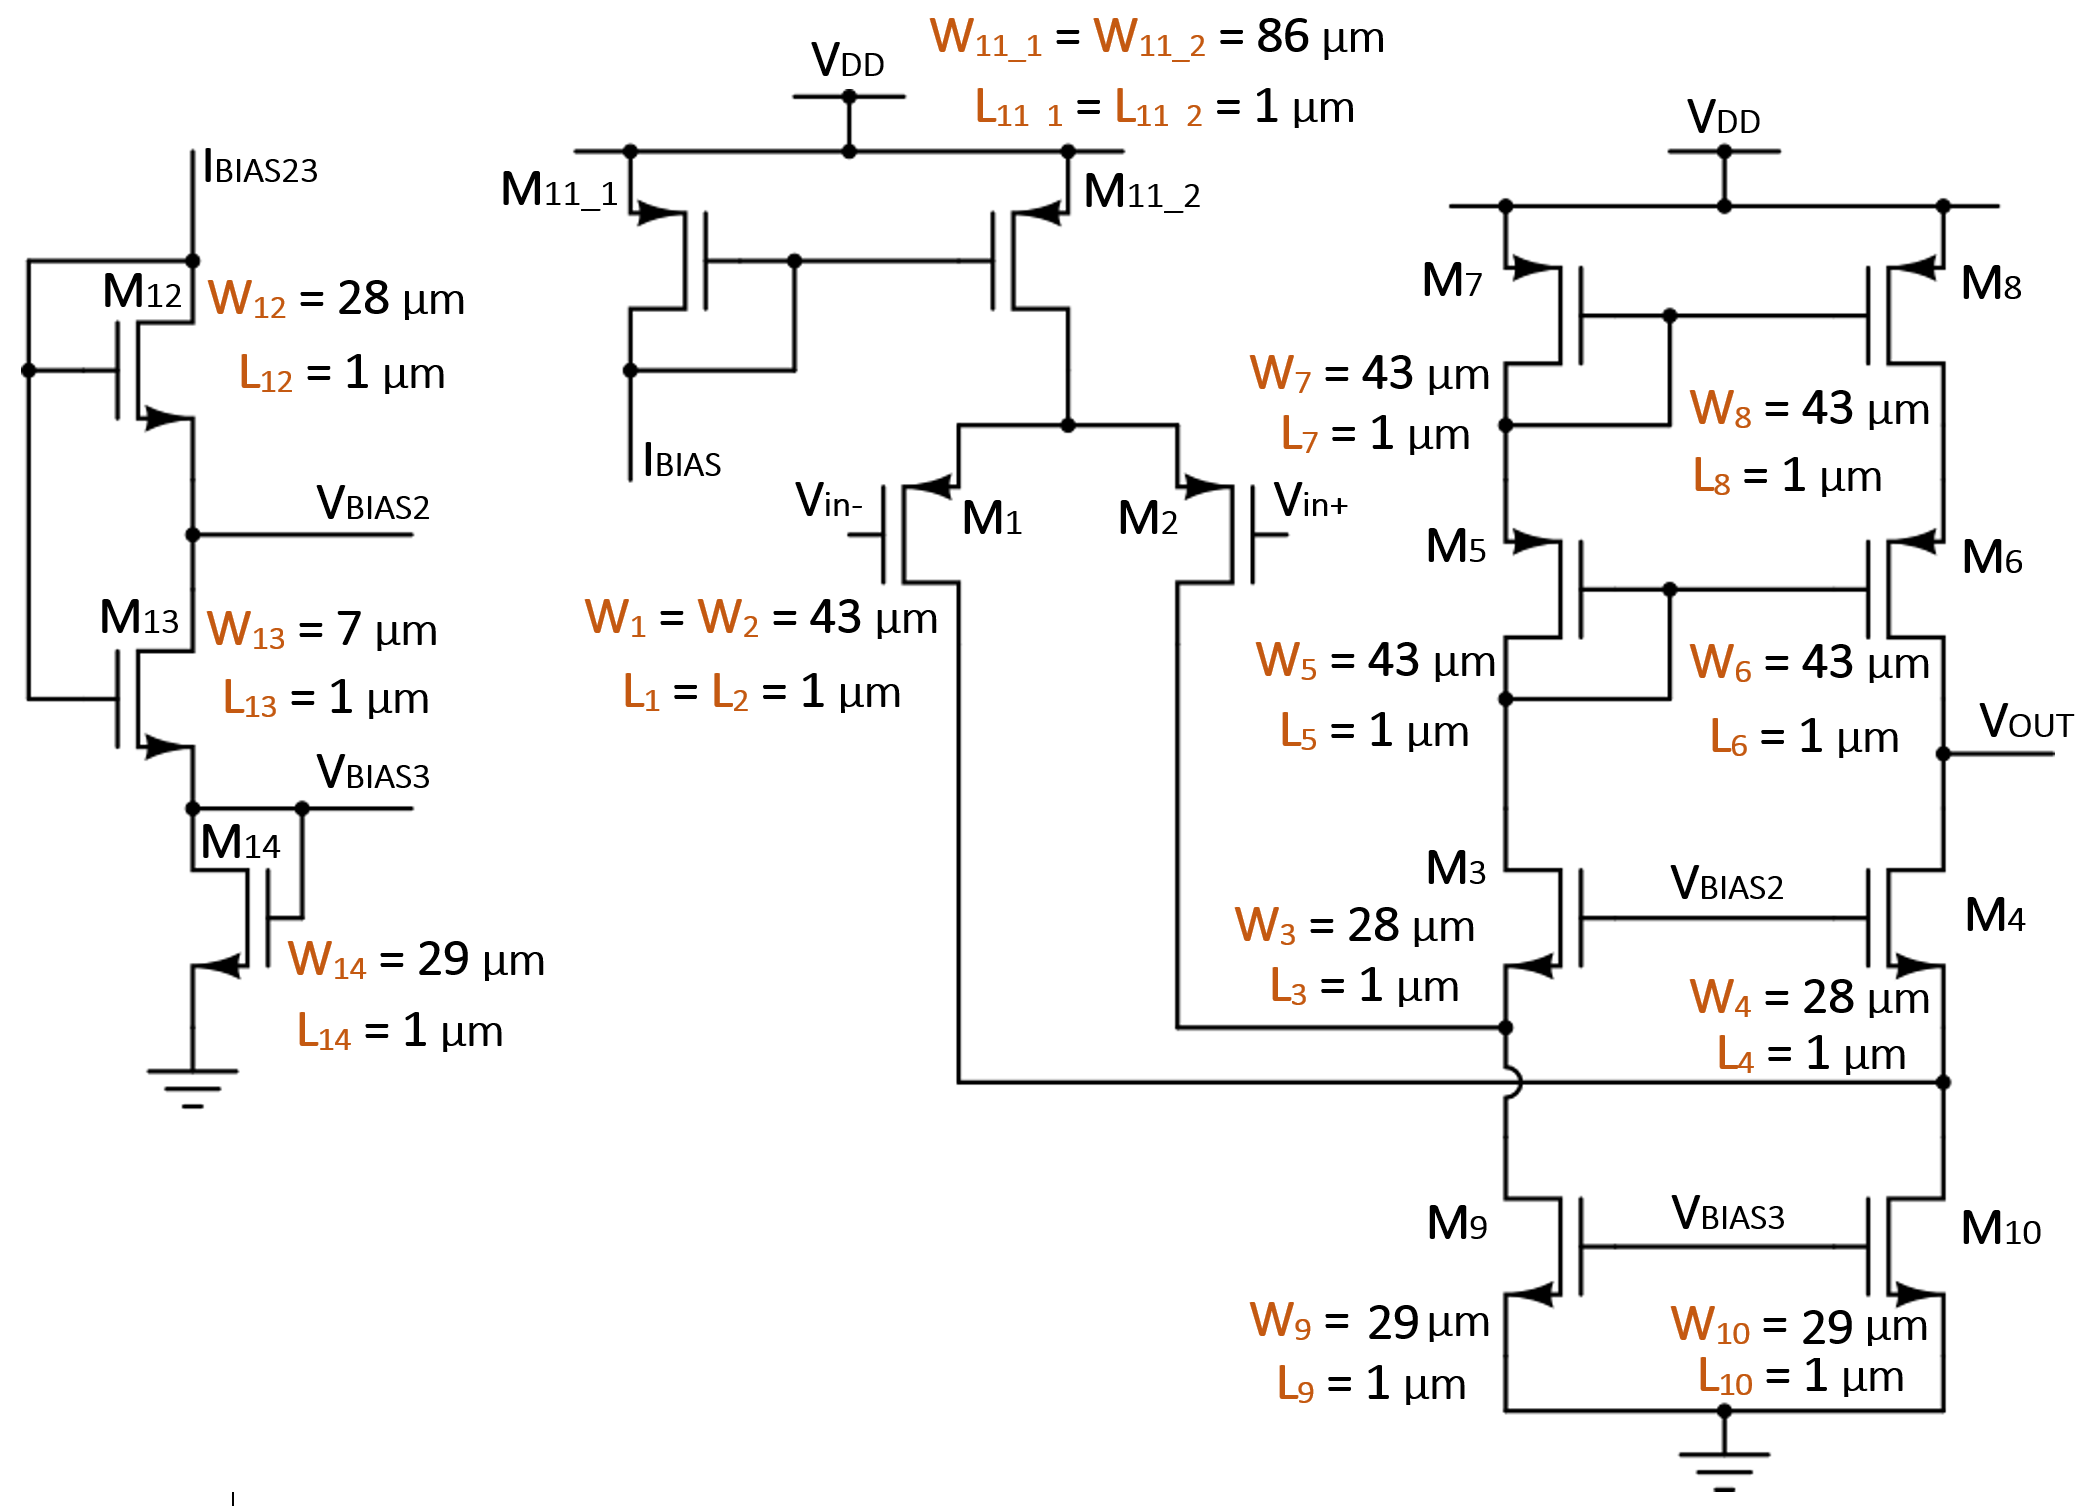
\includegraphics[keepaspectratio=true, scale=0.34]{teoricas/ajuste1}
			\caption{Circuito actual.}
			\vspace{-0.8em}
		\end{figure}
	\end{minipage}
	\begin{minipage}[c]{0.24\textwidth}
		\centering
		\begin{table}[H]
			\centering
			\caption{Especificações.}
			\vspace{-1.5mm}
			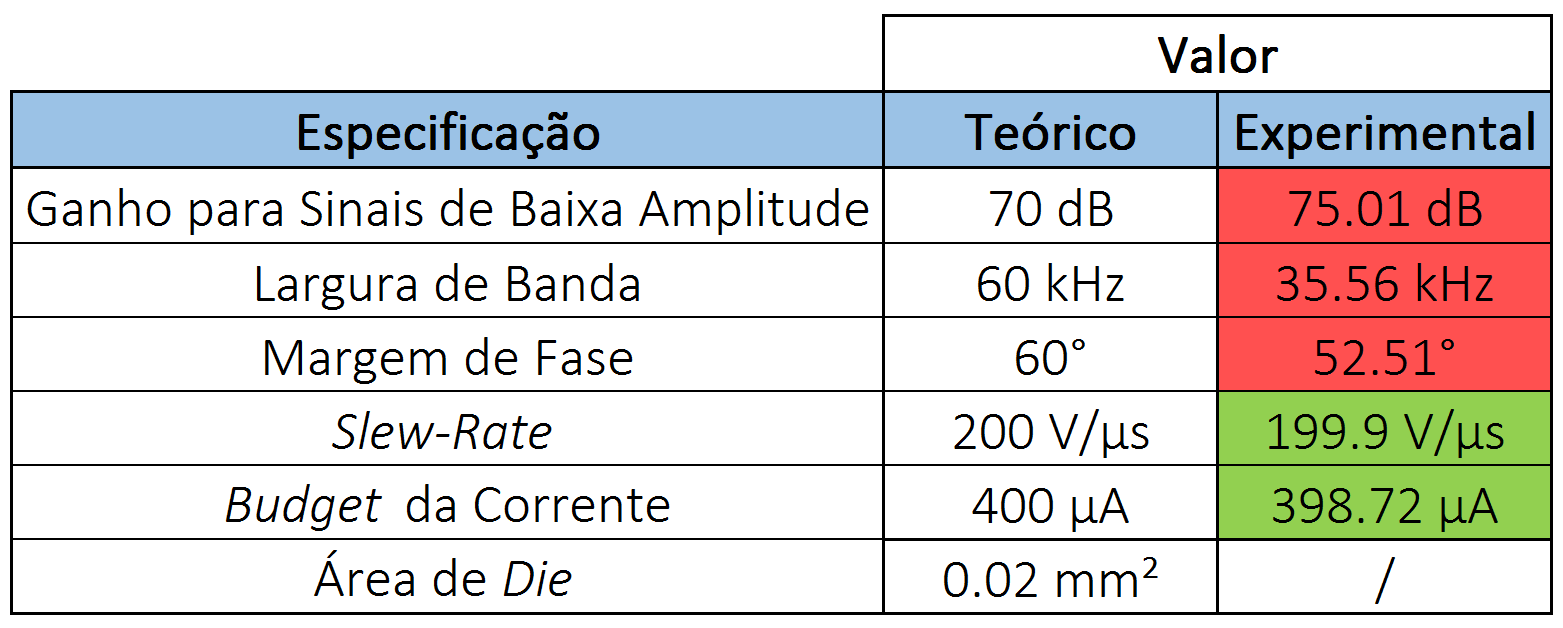
\includegraphics[keepaspectratio=true, scale=0.33]{teoricas/tabajuste1}
		\end{table}
	\end{minipage}	
\end{figure}

\subsection{Ganho e Largura de Banda}

\subsection{Margem de Fase}

\pagebreak

\section{Conclusões}

\end{document}